\chapter{Drupal theming}

In this chapter we are going to learn how to change the look of our site. First we will learn how to change the basic theme settings. Next you will learn how to install a custom theme. The last part of this chapter explains how to extend a theme and add your own html and css.

\section{Theme basics}

\subsection{Changing the theme settings}

To view the settings of your current theme (Bartik) go to \textbf{Appearance $\rightarrow$ Settings}. On his page you can see a tab for each of the enabled themes (Figure \ref{fig:theme_settings_enabled_themes}).

\begin{figure}[H]
	\centering
	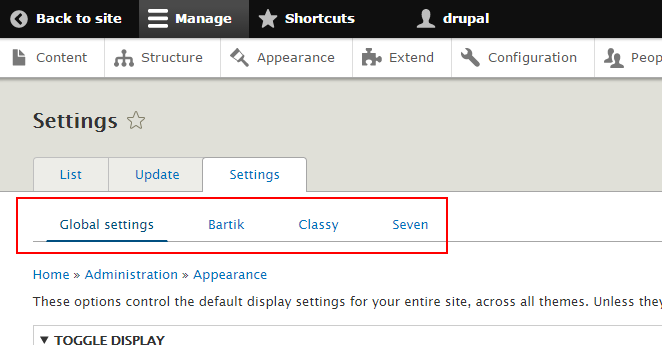
\includegraphics[width=\textwidth]{chapter10/theme_settings_enabled_themes}
	\caption{Theme settings, overview enabled themes.}
	\label{fig:theme_settings_enabled_themes}
\end{figure}

Some themes will come with more settings, such as colour options. Compare the themes you have enabled. Many theme specific settings are very similar to the global settings. When you change settings per theme, they will override the Global settings for that theme. Some of the more interesting themes will offer much more functionality. The default Bartik theme implements functionality from the Colour module, play around with them a little. The Colour module can, but does not have to be implemented in a theme, so not
every theme will offer this functionality.

\begin{figure}[H]
	\centering
	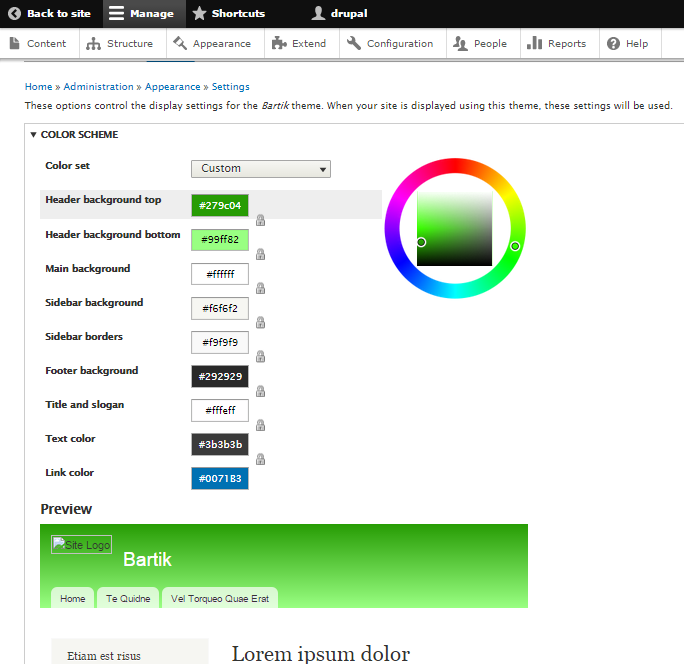
\includegraphics[width=\textwidth]{chapter10/bartik_color_settings}
	\caption{Changing the Bartik color settings.}
	\label{fig:bartik_color_settings}
\end{figure}

Notice in figure \ref{fig:bartik_color_settings} the logo image is not displayed. This is because we are using a custom logo image.

\subsection{Installing a new theme}

In Drupal there are several ways to install a theme. The fist option is to go to \textbf{Appearance $\rightarrow$ Install new theme}. 

\begin{figure}[H]
	\centering
	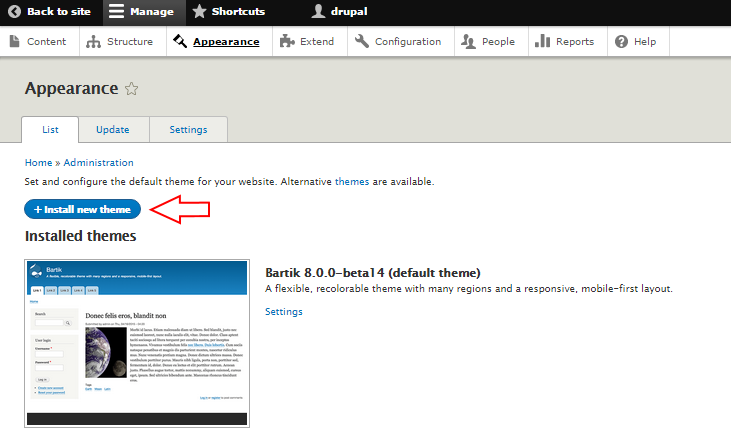
\includegraphics[width=\textwidth]{chapter10/install_new_theme_button}
	\caption{Click the button to install a new theme.}
	\label{fig:install_new_theme_button}
\end{figure}

This will take you to a page where you can either install from a URL, or upload an archive from your local computer.

\begin{figure}[H]
	\centering
	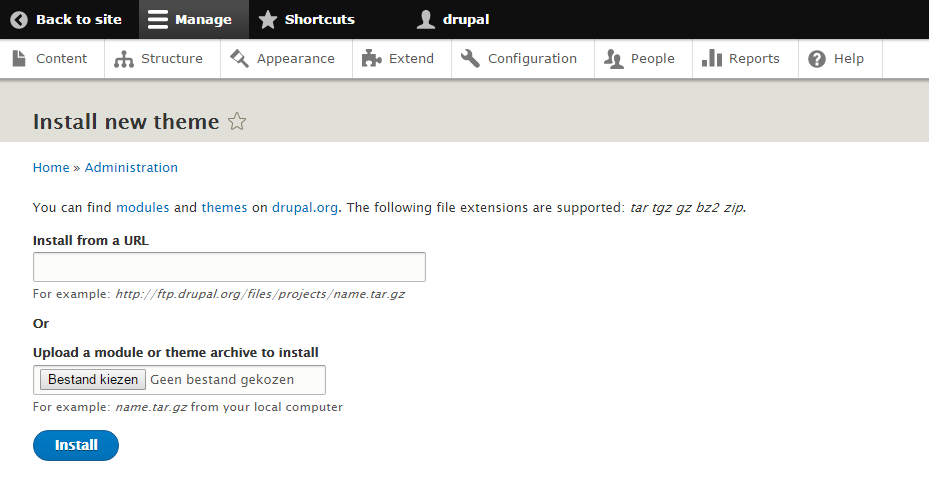
\includegraphics[width=\textwidth]{chapter10/install_new_theme_page}
	\caption{On this page you can choose to install a theme by copying the url from the location where the theme is hosted or uploading the theme from your local computer.}
	\label{fig:install_new_theme_page}
\end{figure}

Either way, you will have to visit the theme project page at \url{https://drupal.org/project/theme_name} and find the file URL for the archive, or just download it, which takes us to option number two.\\

The second way to install a new theme downloading it, unpacking it and placing it in the appropriate folder, which is \url{/themes} (Figure \ref{fig:theme_install_location}). 

\begin{figure}[H]
	\centering
	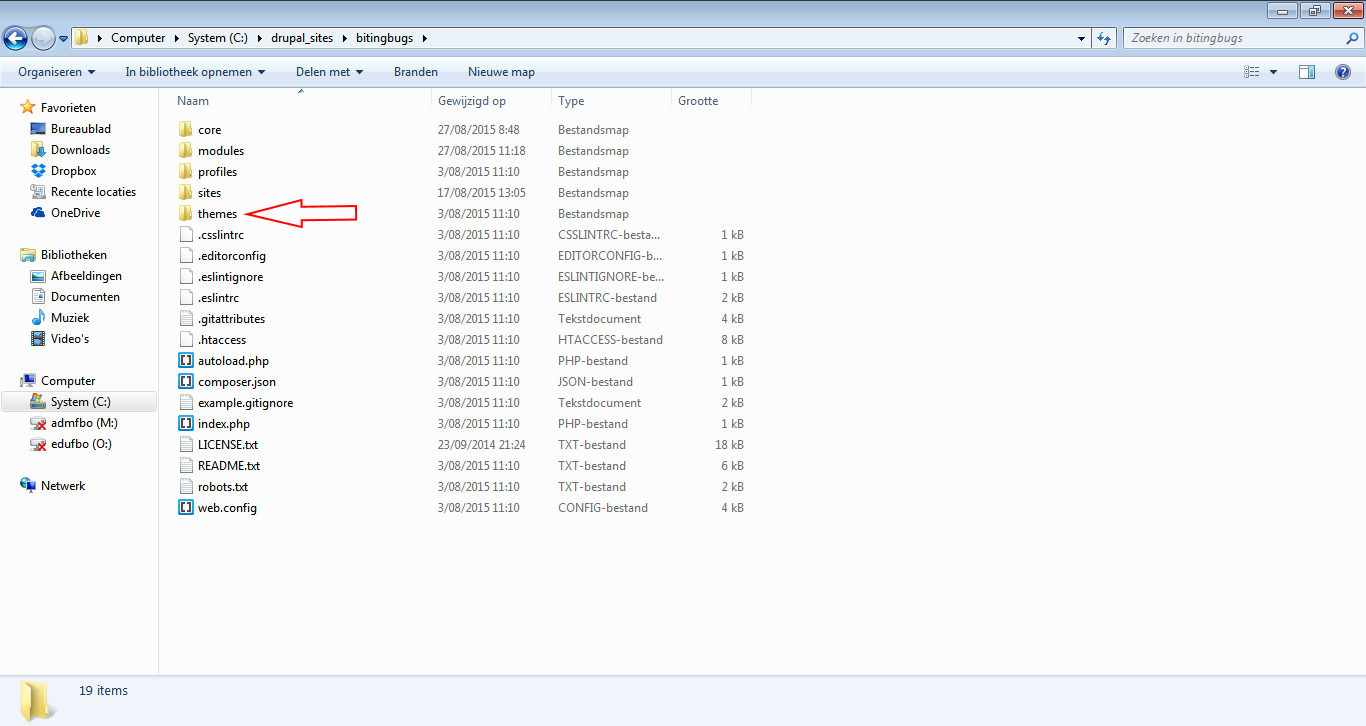
\includegraphics[width=\textwidth]{chapter10/theme_install_location}
	\caption{Theme install location.}
	\label{fig:theme_install_location}
\end{figure}

The third and quickest way to install a theme is through the Drush command line tool. Using Drush we have to type the following two commands:

\begin{lstlisting}[language=bash]
drush dl theme_name
drush en theme_name
\end{lstlisting}

The theme\_name, should be the machine name. This can be found in the URL of the project page on drupal.org, it is the word after project/. For example in \url{www.drupal.org/project/bartik} the machine name is \textbf{bartik}.

Drupal 8 has all core code and themes under a directory named /core. For contributed and custom themes drupal uses the /themes folder that lives on the same level as the /core folder. For people having experience with drupal 7 themes, these are the 2 most apparent changes when we look at a theme folder:
\begin{itemize}
	\item The *.infofile changes to *.info.yml.
	\item The *.tpl.phpfiles change to *.html.twig.
\end{itemize}

The README.txt file in the \url{/themes} directory says the following:\\

\textit{"Place downloaded and custom themes that modify your site's appearance in this directory to ensure clean separation from Drupal core and to facilitate safe, self-contained code updates. Contributed themes from the Drupal community may be downloaded at \url{http://drupal.org/project/themes}.	It is safe to organize themes into subdirectories and is recommended to use	Drupal's sub­theme functionality to ensure easy maintenance and upgrades. In multisite configuration, themes found in this directory are available to all sites. In addition to this directory, shared common themes may also be kept in the \url{sites/all/themes} directory and will take precedence over themes in this directory. Alternatively, the \url{sites/your_site_name/themes} directory pattern may be used to restrict themes to a specific site instance. Refer to the "Appearance" section of the README.txt in the Drupal root directory for further information on theming."
}


\section{Creating your own theme}

To create a new theme navigate to your site \url{/themes} folder. For me this is the \url{C:\drupal_sites\bitingbugs\themes} folder. There we will create a new folder for our theme named \textbf{my\_new\_theme}. Inside the new folder we need a file to describe our theme. Drupal requires this file to be named: \textbf{[theme name].info.yml}. So in our case we create a file named \textbf{my\_new\_theme.info.yml}.

A \url{.yml} file is used for the YAML file type. YAML stands for YAML Ain't Markup Language. It is called this way because it strives to be as human readable as possible. Figure \ref{fig:yaml_file_example} shows an example of a YAML file. As you can see YAML files look very simple because they use whitespace to structure the content. 

\begin{figure}[H]
	\centering
	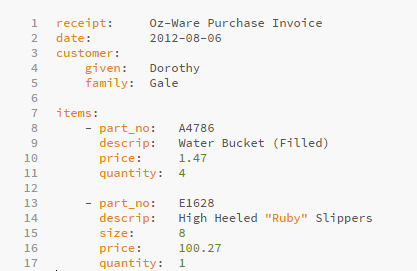
\includegraphics[width=\textwidth]{chapter10/yaml_file_example}
	\caption{An example of a basic YAML file.}
	\label{fig:yaml_file_example}
\end{figure}

The \url{.info.yml} file has four required keys (figure \ref{fig:info_yml_req_keys}):
\begin{description}
	\item[Name:] The human readable name will appear on the Appearance page, where you can activate your theme.
	\item[Type:] The type key indicates the type of extension, e.g. module, theme or profile. For themes this should always be set to "theme".
	\item[Description:] The description is also displayed on the Appearance page.
	\item[Core:] The core key specifies the version of Drupal core that your theme is compatible with.
\end{description}

\begin{figure}[H]
	\centering
	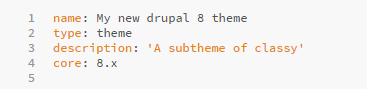
\includegraphics[width=\textwidth]{chapter10/info_yml_req_keys}
	\caption{Required info file keys.}
	\label{fig:info_yml_req_keys}
\end{figure}

Next to the required keys you can also add some other properties:

\begin{description}
	\item[Package:] The package key allows you to group themes together on the Appearance page.
	\item[Base theme:] : The theme can inherit the resources from another theme by defining it as a base theme.
	\item[Version:] For modules hosted on \url{drupal.org}, the version number will be filled in by the packaging script. You should not specify it manually, but leave out the version line entirely.
	\item[Screenshot:] With the screenshot key you define a screenshot that is shown on the	Appearance page. If you do not define this key then Drupal will look for a file named \url{screenshot.png} in the theme folder to display.
	\item[Libraries:] The libraries key can be used to add asset libraries — which can contain both CSS and JS assets — to all pages where the theme is active.
	\item[Stylesheet­remove:] The stylesheets­remove key removes a link to a stylesheet added by another theme or module. The full path to CSS file should be provided (instead of just the filename), to accommodate cases where more than one file with the same name exists. In cases where a Drupal core asset is being removed (for example, a CSS file in jQuery UI) the full file path is needed. In cases where the file is part of a library that belongs to a module or theme, a token can be used. Note that when using the token it needs to be quoted because @ is a reserved indicator in YAML.
	\item[Regions:] Regions are declared as children of the regions key. You are required to have a content region.
\end{description}

Although you only need a \url{.info.yml} file with the required keys to have a new Drupal theme, it will not be of much use. To have a basic functioning theme you should have the following \url{.info.yml} file:

\begin{figure}[H]
	\centering
	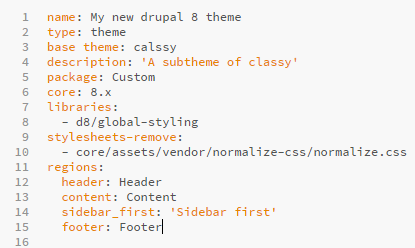
\includegraphics[width=\textwidth]{chapter10/basic_info_yml}
	\caption{A basic info.yml file.}
	\label{fig:basic_info_yml}
\end{figure}

Aside from the \url{.info.yml} file you should also have the \url{html.html.twig} and \url{page.html.twig} template files. A template file defines the structure of a certain part of your Drupal site. They contain html and some logic. However the logic in these files should be limited and is reserved for the \textbf{[theme name].theme} file. You will learn more about template files later in this chapter.

\section{Subtheming}

When we create a subtheme we take an existing theme and use it as a template for our own. The subtheme extends the base theme, this means that we add extra functionality on top of the existing theme. You might be wondering why we don't just modify the base theme. The advantage of extending the base theme is that when it gets updated, our modifications don't get overridden. 

\subsection{How to create a subtheme}

Creating a sub theme is pretty much like creating a theme. The main difference is you (also)
need to declare a parent theme in the *.info.yml file, like so:

\begin{figure}[H]
	\centering
	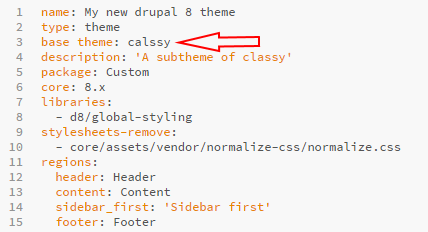
\includegraphics[width=\textwidth]{chapter10/subtheme_declaration}
	\caption{Subtheme declaration in the info.yml file.}
	\label{fig:subtheme_declaration}
\end{figure}

If the base theme has regions and/or features defined in the *.info.yml file which you want to keep, you’ll need to copy those to the sub theme as well. Declaring only your own, will override any existing. Some contributed base themes require a little more to set up, make sure you refer to each theme’s README.txt file for full instructions on how to begin using it, as each is different. As usual with Drupal, there are several ways of doing things. Many of the more popular themes provide Drush integration to make it even easier. So always check the documentation.

When you create a sub theme, it will inherit everything from CSS to the screenshot from the base theme, with the exception of the regions, features and settings defined in the parent’s *.info.yml file. Template files will just work, there’s no need to copy them or create your own, unless you want to override them. In that case, you’ll have to copy the right *.html.twig file in your theme’s templates folder. Functions from the parent’s .theme file will just work, and you can extend/manipulate them further in your own. Since these functions should be prefixed with your theme name, you can use exactly the same hooks to further manipulate data or output.

\subsection{Creating a subtheme in practice}

In this section we will create our own subtheme for the bitingbugs example. First create a folder for our new theme in the \url{/themes} folder (Figure \ref{fig:bitingbugs_subtheme}). 

\begin{figure}[H]
	\centering
	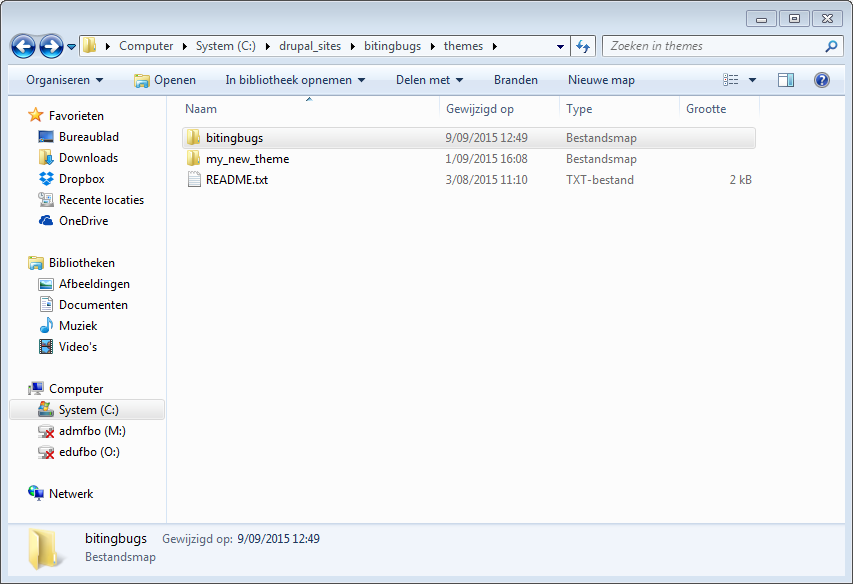
\includegraphics[width=\textwidth]{chapter10/bitingbugs_subtheme}
	\caption{The folder for our new subtheme.}
	\label{fig:bitingbugs_subtheme}
\end{figure}

Next we will add our \url{bitingbugs.info.yml} file to our new theme folder, the file name should have the same name as your theme. This file provides meta­data about your theme to Drupal. This is similar to how modules and installation profiles are being defined, and as such it is important to set the 'type' key in the *.info.yml file to 'theme' in order to differentiate it (Figure \ref{fig:bitingbugs_info_file}).

\begin{figure}[H]
	\centering
	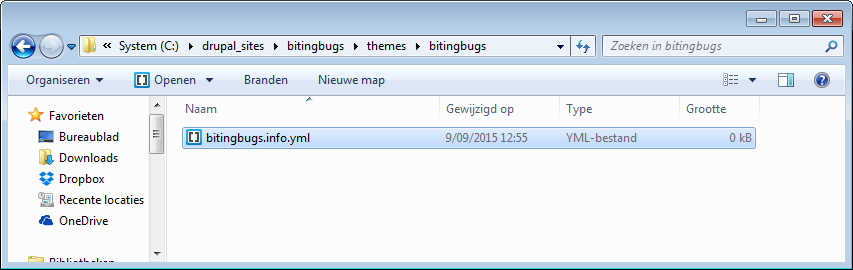
\includegraphics[width=\textwidth]{chapter10/bitingbugs_info_file}
	\caption{Bitingbugs theme info file.}
	\label{fig:bitingbugs_info_file}
\end{figure}

Next we will add some content to our \url{bitingbugs.info.yml} file (Figure \ref{fig:bitingbugs_info_file_content}).

\begin{figure}[H]
	\centering
	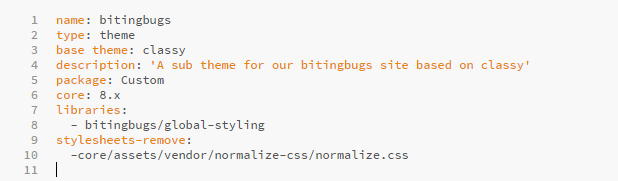
\includegraphics[width=\textwidth]{chapter10/bitingbugs_info_file_content}
	\caption{.info.yml file content.}
	\label{fig:bitingbugs_info_file_content}
\end{figure}

If you have done the previous steps correctly, you should see your theme on the theme settings page of your Drupal site under \textbf{Uninstalled themes}. 

\subsubsection{Adding regions to a sub theme}

Adding regions to a theme requires:
\begin{itemize}
	\item Adding region meta-data to your \url{.info.yml} file.
	\item Editing your \url{page.html.twig} file and printing the new regions.
\end{itemize}

\subsubsection{Adding region meta-data to your .info.yml file}

Start by declaring any new regions in your bitingbugs.info.yml file. Regions are declared as children of the “regions” key like so: 


\begin{figure}[H]
	\centering
	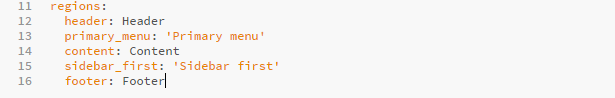
\includegraphics[width=\textwidth]{chapter10/bitingbugs_info_regions}
	\caption{.info.yml regions.}
	\label{fig:bitingbugs_info_regions}
\end{figure}

Region keys can contain: letters, numbers and underscores. Keys should begin with a letter. When referencing regions the key from your bitingbugs.info.yml file will be used as the machine readable name of the region, and is how you will reference the region in code. The human readable name of the region is what will be used in the user interface for anyone administering regions.


\subsubsection{Adding regions to your templates}

In order for regions to display any content placed into them you'll need to make sure your new regions are also added to your page.html.twig file. Regions will be represented as Twig variables whose name corresponds with the key used in your bitingbugs.info.yml file with the string page. prepended. \\
\textbf{Example:}
\begin{lstlisting}
header: 'Header'
\end{lstlisting}
\textbf{Becomes:}
\begin{lstlisting}[language=php]
{{ page.header }}
\end{lstlisting}

\subsubsection{Default regions}
See the page.html.twig documentation for a list of default regions.
	
\begin{itemize}
	\item page.header: Items for the header region.
	\item page.primary\_menu: Items for the primary menu region.
	\item page.secondary\_menu: Items for the secondary menu region.
	\item page highlighted: Items for the highlighted content region.
	\item page.help: Dynamic help text, mostly for admin pages.
	\item page.content: The main content of the current page.
	\item page.sidebar\_first: Items for the first sidebar.
	\item page.sidebar\_second: Items for the second sidebar.
	\item page.footer: Items for the footer region.
	\item page.breadcrumb: Items for the breadcrumb region.
\end{itemize}

Now, main menu, secondary menu and breadcrumb have their own regions. If your theme does not declare any regions Drupal will assume a set of default regions. These regions correspond with what the default \url{core/modules/system/templates/page.html.twig} file expects, as well as two additional regions, page\_top, and page\_bottom, which are output in the default \url{html.html.twig} template.

If you declare any regions in your theme, even just one, all the default regions will no longer be applied and you assume responsibility for declaring any and all regions you want to use. Note: in most cases you'll want to make sure you declare the page\_top and page\_bottom regions in your theme since those are output by the \url{html.html.twig} file and some modules might expect them to be present.

\subsubsection{Review exercise}

Add the copyright region to your bitingbugs subtheme. Enable the theme and see if the regions show up on the block layout page. What do you see?


\section{TWIG templates}

Twig is a PHP­based compiled templating language. When your web page renders, the Twig engine takes the template and converts it into a 'compiled' PHP template which it stores in a protected directory in \url{sites/default/files/php_storage/...} The compilation is done once. Template files are cached for reuse and are recompiled on clearing the Twig cache.

\subsection{Working with Twig templates}
Drupal allows you to override all of the templates that are used to produce HTML markup so that you can fully control the markup that is being output within a custom theme. There are templates for each page element ranging from the high level HTML to small fields.

\subsection{Overriding templates}

You can override Drupal core templates by adding templates to your theme folder that follow a specific naming convention. To override templates you:
\begin{itemize}
	\item Locate the template you wish to override.
	\item Copy the template file from its base location into your theme folder.
	\item (optionally) Rename the template according to the naming conventions in order to target a more specific subset of areas where the template is used.
	\item Modify the template to your liking.
\end{itemize}

Once you copy a template file into your theme and clear the cache Drupal will start using your instance of the template file instead of the base version. You can find out what templates are in use for any part of the page by using the Twig debugging tools.

\subsubsection{Rebuild cache}

When working with theme hook suggestions, there is a possibility that Drupal uses its cache rather than the new templates as suggested. Clear the cache if you experience this problem. To clear the cache, you can do this through the interface, or with drush. The drush command has been changed and is now \textit{drush cache-­rebuild} or \textit{drush cr} for short.

\subsubsection{Overview of the template naming conventions}

Say we want to add a template override for a page, drupal will look at the path and for example see \url{http://mysite.com/node/1}. Drupal will split this path up into components. In this case the components are \textbf{node} and \textbf{1}. And because we want to change a template for an entire page, the prefix will be \textit{page}. When the prefix is chosen drupal goes through the components to decide possible template names. For example if we want to change the \textit{page} template for the \url{http://mysite.com/node/1} url we can change the following templates:

\begin{enumerate}
	\item page.html.twig (This will change the template for all pages)
	\item page--node.html.twig (This changes the template for all /node pages)
	\item page--node--\%.html.twig (This will change the template for all /node pages as well)
	\item page--node--1.html.twig (This will change the template for the node with id 1)
	\item page--front.html.twig (This will only change node/1 if it is the front page)
\end{enumerate}

When the page is actually rendered, the last possibility is checked. If it exists, that possibility is used. Otherwise the next possibility up is checked, and so on. Of course, if none of the overriding possibilities exist, page.html.twig is the final possibility. This also explains why page--­­front.html.twig, if it exists, overrides any other possibilities for the front page: it is always the last possibility for the page designated as the front page. Besides page templates we can add a number of other templates to override more specific html, here’s a list with examples of template names:

\begin{description}
	\item[HTML] The HTML template provides markup for the basic structure of the HTML­page including the \textless head\textgreater, \textless title\textgreater  and \textless body\textgreater  tags.
	Base template: html.html.twig (base location: \url{core/modules/system/templates/html.html.twig}) 
	Here is an example of how you may override the base template:
	html--node--id.html.twig
	
	\item[Page] Pattern: page--[front|internal/path].html.twig
	Base template: page.html.twig (base location:
	\url{core/modules/system/templates/page.html.twig})
	\url{http://mysite.com/node/1/edit} would result in the following suggestions:
	\begin{enumerate}
		\item page--node--edit.html.twig
		\item page--node--1.html.twig
		\item page--node.html.twig
		\item page.html.twig
	\end{enumerate}
	
	\item[Regions] Pattern: region--[region].html.twig
	Base template: region.html.twig (base location:
	\url{core/modules/system/templates/region.html.twig})


	\item[Blocks] Pattern: block--[module[--­delta]].html.twig
	Base template: block.html.twig (base location: \url{core/modules/block/templates/block.html.twig})
	\textit{module} being the name of the module and \textit{delta}, the internal id assigned to the block by the module.
	If you have a block created by views module with a view name \textit{front\_news} and display id \textit{block\_1} then the template would be:
	block--views-block--front-news-block-1.html.twig (notice, when you have underscores in a display id or in a view name ­ you have to transform them into a single dash) Be aware that module names are case sensitive in this context. For instance if your module is called \textit{MyModule}, the most general template for this module would be
	\textit{block--MyModule.html.twig}.
	
	\item[Nodes] Pattern: node--[type|nodeid].html.twig
	Base template: node.html.twig (base location: \url{core/modules/node/templates/node.html.twig})
	Template names are made based on these factors, listed from the most specific template to
	the least. Drupal will use the most specific template it finds:
	\begin{enumerate}
		\item node--nodeid.html.twig
		\item node--type.html.twig
		\item node.html.twig
	\end{enumerate}
	Note that underscores in a content type's machine name are replaced by hyphens.

	\item[Taxonomy terms] Pattern: taxonomy-term--[vocabulary-machine-name|tid].html.twig
	Base template: taxonomy-term.html.twig (base location:
	\url{core/modules/taxonomy/templates/taxonomy­term.html.twig})
	Template names are made based on these factors, listed from the most specific template to the least. Drupal will use the most specific template it finds:
	\begin{enumerate}
		\item taxonomy-term--tid.html.twig
		\item taxonomy-term--vocabulary-machine-name.html.twig
		\item taxonomy-term.html.twig
	\end{enumerate}
	Note that underscores in a vocabulary's machine name are replaced by hyphens.

	\item[Fields] Pattern: field--[type|name[--content-type]|content-type].html.twig
	Base template: field.html.twig (base location: \url{core/modules/system/templates/field.html.twig})
	Template names are made based on these factors, listed from the most specific template to the least. Drupal will use the most specific template it finds:
	\begin{enumerate}
		\item field--field-name--content-type.html.twig
		\item field--content-type.html.twig
		\item field--field-name.html.twig
		\item field--field-type.html.twig
	\end{enumerate}
	Note that underscores in a Field's machine name are replaced by hyphens. Also remember to include \textit{field} in custom field names, e.g: field--field-phone.html.twig

	\item[Comments] Pattern: comment--node-[type].html.twig
	Base template: comment.html.twig (base location:
	\url{core/modules/comment/template/comment.html.twig}
	
	\item[Forums] Pattern: forums--[[container|topic]--forumID].html.twig
	Base template: forums.html.twig (base location: \url{core/modules/forum/templates/forums.html.twig}).
	
	\item[Maintenance page] Pattern: maintenance-page--[offline].html.twig
	Base template maintenance-page.html.twig (base location: \url{core/modules/system/templates/maintenance­page.html.twig}).
	
	\item[Search result] Pattern: search-result--[searchType].html.twig
	Base template: search-result.html.twig (base location: \url{core/modules/search/templates/search­result.html.twig}).


\end{description}

\subsection{The template file contents}

Have a look at the \url{page.html.twig} template. You can find it at \url{core/themes/classy/templates/layout/}. In figure \ref{fig:page_template_header} you can see the header.

\begin{figure}[H]
	\centering
	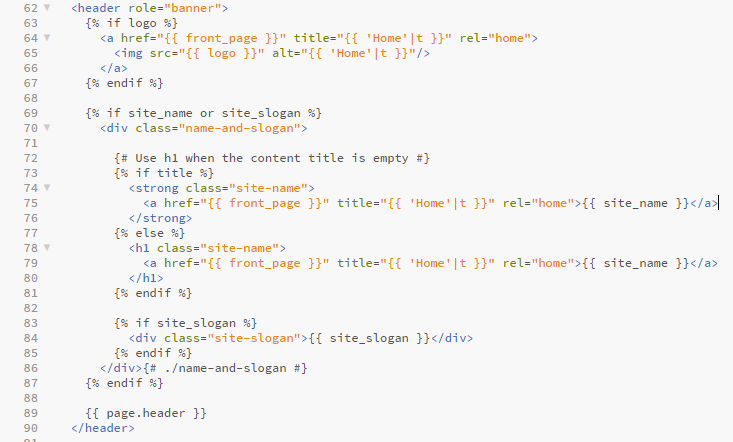
\includegraphics[width=\textwidth]{chapter10/page_template_header}
	\caption{page.html.twig content.}
	\label{fig:page_template_header}
\end{figure}

As you can see a template file is made up of standard html and some strange tags. The Twig engine is responsible for interpreting these tags. There are three types of tags:
\begin{itemize}
	\item $\{\{\ These\ \}\}$ are for printing content, either explicitly or via functions.
	\item $\{\%\ These\ \%\}$ are for executing statements.
	\item $\{\#\ These\ \#\}$ are for comments.
\end{itemize}

\subsection{Printing variables and regions}

\begin{figure}[H]
	\centering
	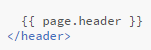
\includegraphics[width=\textwidth]{chapter10/printing_varibles_and_regions}
	\caption{Printing variables and regions.}
	\label{fig:printing_varibles_and_regions}
\end{figure}

\subsection{Executing statements}

\begin{figure}[H]
	\centering
	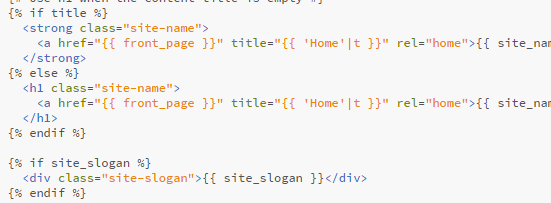
\includegraphics[width=\textwidth]{chapter10/executing_statements}
	\caption{Executing statements.}
	\label{fig:executing_statements}
\end{figure}

\subsection{Comments}

\begin{figure}[H]
	\centering
	
\includegraphics[width=\textwidth]{chapter10/comments}
	\caption{Comments}
	\label{fig:comments}
\end{figure}

\subsection{Overriding a template}
In this section we are going to override the page template in our bitingbugs theme. Copy the template file \url{page.html.twig} from \url{/core/themes/classy/templates/layout/} to \url{/themes/bitingbugs/templates/layout/}. Open the template file. You can see that the different regions that we defined in our .info.yml file are printed in certain locations on this page. If you remember, our \textbf{copyright} region did not show up on the regions page. To make it show up we will have to add it to our page template. Add The following code above the closing main tag:

\begin{figure}[H]
	\centering
	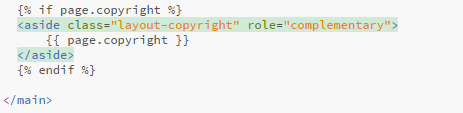
\includegraphics[width=\textwidth]{chapter10/copyright_region}
	\caption{Copyright region}
	\label{fig:copyright_region}
\end{figure}


Clear the drupal caches and to the block region demonstration on your site. There you will see the \textbf{Copyright} region show up between the \textbf{Sidebar first} and \textbf{Footer} regions.

Next we will wrap the footer content into a div container so we can give it af full width layout later:

\begin{figure}[H]
	\centering
	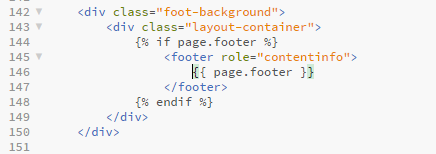
\includegraphics[width=\textwidth]{chapter10/page_footer_wrapper}
	\caption{Page footer wrapper.}
	\label{fig:page_footer_wrapper}
\end{figure}

\subsection{Twig filters}
Filters in Twig can be used to modify variables. Filters are separated from the variable by a pipe symbol (|) and may have optional arguments in parentheses. Multiple filters can be chained. The output of one filter is applied to the next.
Example: {{ ponies|safe\_join(", ")|lower}}
The list of filters that can be used in Twig templates for Drupal consists of all the filters in the Twig engine as well as some Drupal specific filters.

\subsubsection{Translation filters}

The t filter will run the variable through the Drupal t() function, which will return a translated string. This filter should be used for any interface strings manually placed in the template that will appear for users.

\begin{figure}[H]
	\centering
	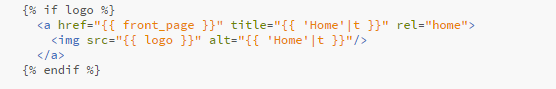
\includegraphics[width=\textwidth]{chapter10/translation_filter}
	\caption{Translation filter.}
	\label{fig:translation_filter}
\end{figure}

This means that if we add this filter, we should be able to translate this string in the translation interface.

\subsubsection{passthrough, and placeholder}

In order to safely escape all of the Twig variables detected in an {\% trans \%} tag, the variables are sent with an @ prefix by default. To pass­through a variable (!) or use as a placeholder (\%), the passthrough or placeholder filters are used. Passthrough gets no sanitization or formatting and should only be used for text that has already been prepared for HTML display. placeholder gets escaped to HTML and formatted using drupal\_placeholder(), which makes it display as emphasized text.



\section{Debugging Twig templates}

The Twig engine provides options for configuring debugging, automatic reloading (recompiling) of templates, and caching compiled templates in the filesystem. By default, the Twig theming engine compiles templates into PHP code and stores the compiled code in memory. Compiled code is unsuitable for development, since changes in Twig templates are not immediately updated in your Drupal site. Twig cache can be cleared through Drupal's clear cache interface, but for ongoing development it's easier to change Drupal's settings so that Twig doesn't cache anything at all.
The Drupal 8 implementation also adds an additional tool that allows you to locate the template that outputs the markup.

\subsection{Enable debugging}

To enable debugging locate the \url{/sites/default/default.services.yml} file. Copy this file and rename it to services.yml. Edit the services.yml file and change the following parameters:


\begin{description}
	\item[debug] true (Turn on debugging)
	\item[auto\_reload] true (Automatically recompile Twig templates when the source changes)
	\item[cache] false (Disable caching)
\end{description}

Now clear the drupal cache. Go to \textbf{Configuration $\rightarrow$ Development $\rightarrow$ Performance $\rightarrow$ Clear Cache} or use the \textbf{drush cache-rebuild} command.

\section{Review exercises}

In this exercise you are going to create a new subtheme for our bitingbugs example. Our new theme will be based on the Bartik theme.
\begin{enumerate}
	\item Now create a new folder for your theme and put the correct .info.yml file inside. You can use the default Bartik regions.
	\item enable your new subtheme.
	\item Move the \textbf{Powered by drupal}, \textbf{User account menu}, \textbf{Footer menu}, \textbf{Help}, \textbf{Tools} and \textbf{User login} blocks to the \textbf{None} region.
	\item We would like to change the size of the recipe titles on the homepage. Use your browser's development tools to locate the twig template where the title is generated. Override the template and wrap the title inside H2 tags.
	\begin{figure}[H]
		\centering
		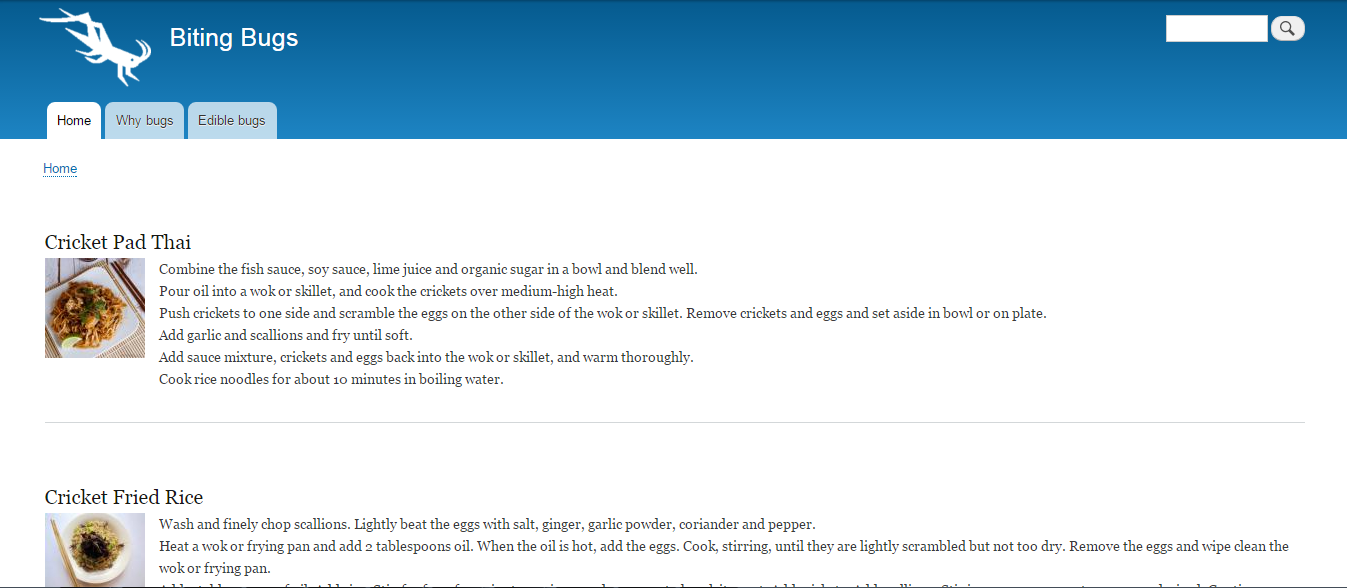
\includegraphics[width=\textwidth]{chapter10/bitingbugs_updated_title_size}
		\caption{We changed the title by wrapping it in an H2 tag.}
		\label{fig:bitingbugs_updated_title_size}
	\end{figure}
	\item Next we are going to change the recipe page. Click one of the recipe titles on the homepage. Inspect the html behind the ingredients list. 
	\begin{figure}[H]
		\centering
		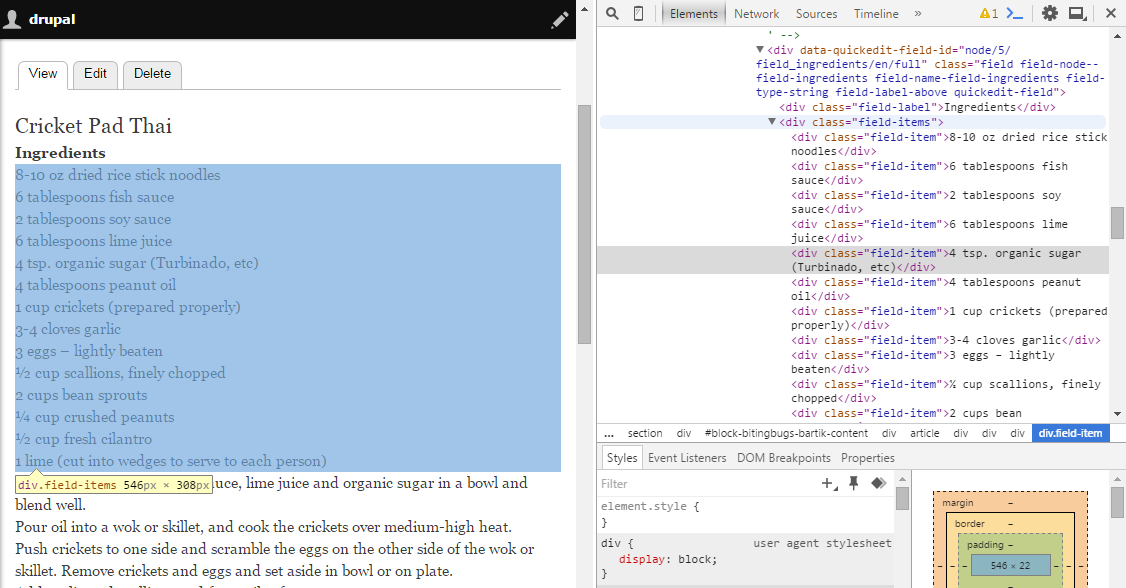
\includegraphics[width=\textwidth]{chapter10/bitingbugs_ingredients_list}
		\label{fig:bitingbugs_ingredients_list}
	\end{figure}
	As you can see right now the ingredients list is a DIV element with another DIV for each recipe. Override the right template to change it to an html list. The resulting HTML should look like this:
	\begin{figure}[H]
		\centering
		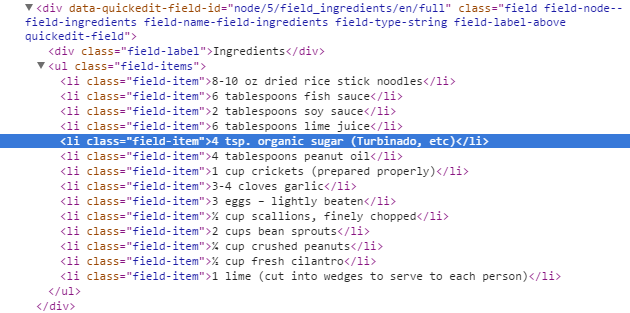
\includegraphics[width=\textwidth]{chapter10/bitingbugs_ingredients_list_list}
		\label{fig:bitingbugs_ingredients_list_list}
	\end{figure}
	\item HINT: make sure you always use the most specific filename for your overridden template
	\item HINT: Use the debug comments to locate the correct template file to override.
\end{enumerate}


\section{CSS and JavaScript}
























